\subsection{Aufbau der Batterie mit Schutzschaltung}
Die beiden originalen Bleibatterien des \textsc{Detroits} hatten eine Nennspannung von $42$ V, was 21 in Serie geschalteten Zellen entspricht. Diese Spannung sollte mit den Lithium Akkus grob erreicht werden, wobei eine Abweichung von $\pm 10$ \% vertretbar ist. Im Idealfall wäre es dabei möglich, die Zellen in den bereits bestehenden Viererrahmen mit einer Nennspannung von $4\cdot 3.7$ V$=14.8$ V zu belassen.

Mit drei in Serie geschalteten Viererrahmen ergibt sich eine Spannung von $3\cdot 4\cdot 3.7$ V$=44.8$ V, was die Bedingung sehr gut erfüllt. Somit können sämtliche Zellen in den Viererrahmen belassen werden, sodass im Folgenden nur noch die Viererrahmen (vier Zellen sind jeweils bereits in einem Gehäuse) behandelt werden. Zuerst soll Tabelle \ref{tab:bat_vergl} einen Vergleich über die Spannungen der beiden Batterien geben:

\begin{table}[h]
\centering
\begin{tabular}{|l|l|l|}
\hline
\textbf{Batterietyp}              & \textbf{Bleiakkumulator} & \textbf{Lithium-Ionen-Akkumulator} \\ \hline
\textbf{Nennspannung Einzelzelle} & $2.0$ V                            & $3.7$ V                                    \\ \hline
\textbf{Anzahl Serieschaltung}    & 21                                  & 12                                          \\ \hline
\textbf{Minimalspannung Batterie} & $21\cdot1.8$ V$=37.8$ V           & $12\cdot2.8$ V$=33.6$ V                     \\ \hline
\textbf{Nennspannung Batterie}    & $21\cdot2.0$ V$=42.00$ V           & $12\cdot3.7$ V$=44.4$ V                    \\ \hline
\textbf{Maximalspannung Batterie} & $21\cdot2.4$ V$=50.40$ V            & $12\cdot4.1$ V$=49.2$ V                     \\ \hline
\end{tabular}
\caption{Vergleich des originalen Bleiakkumulators mit dem neuen Lithium-Ionen-Akkumulator}
\label{tab:bat_vergl}
\end{table}

Interessanterweise sind sowohl Lade- als auch Entladeschlussspannung der neuen Batterie etwas tiefer als die vergleichbaren Werte des Bleiakkus, obwohl die Nennspannung höher ist. Dies liegt an der wesentlich flacheren Entladekurve des Lithium-Ionen-Akkus im Vergleich zum Bleiakku. Mit diesen Werten kann aber gezeigt werden, dass die Spannungen der neuen Batterie sehr gut zu denen des Originals passen.

Insgesamt waren 22 Viererrahmen vorhanden. Mit dem Ziel von zwei Batterien mit je drei Viererrahmen in Serie kann man so pro Batterie eine dreifache Parallelschaltung machen. Dies benötigt insgesamt 18 Viererrahmen, wobei vier übrig bleiben. Der verwendete Aufbau der Batterien ist in Abbildung \ref{fig:schema_batterie} gezeigt, wobei jeweils die senkrecht unter einander stehenden Zellen in Serie geschaltet sind:

\begin{figure}[h]
	\centering
	\footnotesize
\begin{tabular}{lp{2mm}lp{2mm}lp{1.5cm}lp{2mm}lp{2mm}l}
\cline{1-1} \cline{3-3} \cline{5-5} \cline{7-7} \cline{9-9} \cline{11-11}
\multicolumn{1}{|l|}{BAT111.1} & \multicolumn{1}{l|}{} & \multicolumn{1}{l|}{BAT121.1} & \multicolumn{1}{l|}{} & \multicolumn{1}{l|}{BAT131.1} & \multicolumn{1}{l|}{} & \multicolumn{1}{l|}{BAT241.1} & \multicolumn{1}{l|}{} & \multicolumn{1}{l|}{BAT251.1} & \multicolumn{1}{l|}{} & \multicolumn{1}{l|}{BAT261.1} \\ \cline{1-1} \cline{3-3} \cline{5-5} \cline{7-7} \cline{9-9} \cline{11-11} 
\multicolumn{1}{|l|}{BAT111.2} & \multicolumn{1}{l|}{} & \multicolumn{1}{l|}{BAT121.2} & \multicolumn{1}{l|}{} & \multicolumn{1}{l|}{BAT131.2} & \multicolumn{1}{l|}{} & \multicolumn{1}{l|}{BAT241.2} & \multicolumn{1}{l|}{} & \multicolumn{1}{l|}{BAT251.2} & \multicolumn{1}{l|}{} & \multicolumn{1}{l|}{BAT261.2} \\ \cline{1-1} \cline{3-3} \cline{5-5} \cline{7-7} \cline{9-9} \cline{11-11} 
\multicolumn{1}{|l|}{BAT111.3} & \multicolumn{1}{l|}{} & \multicolumn{1}{l|}{BAT121.3} & \multicolumn{1}{l|}{} & \multicolumn{1}{l|}{BAT131.3} & \multicolumn{1}{l|}{} & \multicolumn{1}{l|}{BAT241.3} & \multicolumn{1}{l|}{} & \multicolumn{1}{l|}{BAT251.3} & \multicolumn{1}{l|}{} & \multicolumn{1}{l|}{BAT261.3} \\ \cline{1-1} \cline{3-3} \cline{5-5} \cline{7-7} \cline{9-9} \cline{11-11} 
\multicolumn{1}{|l|}{BAT111.4} & \multicolumn{1}{l|}{} & \multicolumn{1}{l|}{BAT121.4} & \multicolumn{1}{l|}{} & \multicolumn{1}{l|}{BAT131.4} & \multicolumn{1}{l|}{} & \multicolumn{1}{l|}{BAT241.4} & \multicolumn{1}{l|}{} & \multicolumn{1}{l|}{BAT251.4} & \multicolumn{1}{l|}{} & \multicolumn{1}{l|}{BAT261.4} \\ \cline{1-1} \cline{3-3} \cline{5-5} \cline{7-7} \cline{9-9} \cline{11-11} 
                               &                       &                               &                       &                               &                       &                               &                       &                               &                       &                               \\ \cline{1-1} \cline{3-3} \cline{5-5} \cline{7-7} \cline{9-9} \cline{11-11} 
\multicolumn{1}{|l|}{BAT112.1} & \multicolumn{1}{l|}{} & \multicolumn{1}{l|}{BAT122.1} & \multicolumn{1}{l|}{} & \multicolumn{1}{l|}{BAT132.1} & \multicolumn{1}{l|}{} & \multicolumn{1}{l|}{BAT242.1} & \multicolumn{1}{l|}{} & \multicolumn{1}{l|}{BAT252.1} & \multicolumn{1}{l|}{} & \multicolumn{1}{l|}{BAT262.1} \\ \cline{1-1} \cline{3-3} \cline{5-5} \cline{7-7} \cline{9-9} \cline{11-11} 
\multicolumn{1}{|l|}{BAT112.2} & \multicolumn{1}{l|}{} & \multicolumn{1}{l|}{BAT122.2} & \multicolumn{1}{l|}{} & \multicolumn{1}{l|}{BAT132.2} & \multicolumn{1}{l|}{} & \multicolumn{1}{l|}{BAT242.2} & \multicolumn{1}{l|}{} & \multicolumn{1}{l|}{BAT252.2} & \multicolumn{1}{l|}{} & \multicolumn{1}{l|}{BAT262.2} \\ \cline{1-1} \cline{3-3} \cline{5-5} \cline{7-7} \cline{9-9} \cline{11-11} 
\multicolumn{1}{|l|}{BAT112.3} & \multicolumn{1}{l|}{} & \multicolumn{1}{l|}{BAT122.3} & \multicolumn{1}{l|}{} & \multicolumn{1}{l|}{BAT132.3} & \multicolumn{1}{l|}{} & \multicolumn{1}{l|}{BAT242.3} & \multicolumn{1}{l|}{} & \multicolumn{1}{l|}{BAT252.3} & \multicolumn{1}{l|}{} & \multicolumn{1}{l|}{BAT262.3} \\ \cline{1-1} \cline{3-3} \cline{5-5} \cline{7-7} \cline{9-9} \cline{11-11} 
\multicolumn{1}{|l|}{BAT112.4} & \multicolumn{1}{l|}{} & \multicolumn{1}{l|}{BAT122.4} & \multicolumn{1}{l|}{} & \multicolumn{1}{l|}{BAT132.4} & \multicolumn{1}{l|}{} & \multicolumn{1}{l|}{BAT242.4} & \multicolumn{1}{l|}{} & \multicolumn{1}{l|}{BAT252.4} & \multicolumn{1}{l|}{} & \multicolumn{1}{l|}{BAT262.4} \\ \cline{1-1} \cline{3-3} \cline{5-5} \cline{7-7} \cline{9-9} \cline{11-11} 
                               &                       &                               &                       &                               &                       &                               &                       &                               &                       &                               \\ \cline{1-1} \cline{3-3} \cline{5-5} \cline{7-7} \cline{9-9} \cline{11-11} 
\multicolumn{1}{|l|}{BAT113.1} & \multicolumn{1}{l|}{} & \multicolumn{1}{l|}{BAT123.1} & \multicolumn{1}{l|}{} & \multicolumn{1}{l|}{BAT133.1} & \multicolumn{1}{l|}{} & \multicolumn{1}{l|}{BAT243.1} & \multicolumn{1}{l|}{} & \multicolumn{1}{l|}{BAT253.1} & \multicolumn{1}{l|}{} & \multicolumn{1}{l|}{BAT263.1} \\ \cline{1-1} \cline{3-3} \cline{5-5} \cline{7-7} \cline{9-9} \cline{11-11} 
\multicolumn{1}{|l|}{BAT113.2} & \multicolumn{1}{l|}{} & \multicolumn{1}{l|}{BAT123.2} & \multicolumn{1}{l|}{} & \multicolumn{1}{l|}{BAT133.2} & \multicolumn{1}{l|}{} & \multicolumn{1}{l|}{BAT243.2} & \multicolumn{1}{l|}{} & \multicolumn{1}{l|}{BAT253.2} & \multicolumn{1}{l|}{} & \multicolumn{1}{l|}{BAT263.2} \\ \cline{1-1} \cline{3-3} \cline{5-5} \cline{7-7} \cline{9-9} \cline{11-11} 
\multicolumn{1}{|l|}{BAT113.3} & \multicolumn{1}{l|}{} & \multicolumn{1}{l|}{BAT123.3} & \multicolumn{1}{l|}{} & \multicolumn{1}{l|}{BAT133.3} & \multicolumn{1}{l|}{} & \multicolumn{1}{l|}{BAT243.3} & \multicolumn{1}{l|}{} & \multicolumn{1}{l|}{BAT253.3} & \multicolumn{1}{l|}{} & \multicolumn{1}{l|}{BAT263.3} \\ \cline{1-1} \cline{3-3} \cline{5-5} \cline{7-7} \cline{9-9} \cline{11-11} 
\multicolumn{1}{|l|}{BAT113.4} & \multicolumn{1}{l|}{} & \multicolumn{1}{l|}{BAT123.4} & \multicolumn{1}{l|}{} & \multicolumn{1}{l|}{BAT133.4} & \multicolumn{1}{l|}{} & \multicolumn{1}{l|}{BAT243.4} & \multicolumn{1}{l|}{} & \multicolumn{1}{l|}{BAT253.4} & \multicolumn{1}{l|}{} & \multicolumn{1}{l|}{BAT263.4} \\ \cline{1-1} \cline{3-3} \cline{5-5} \cline{7-7} \cline{9-9} \cline{11-11} 
\end{tabular}
	\caption{Aufbau der Batterien; senkrecht = Serieschaltung; waagerecht = Parallelschaltung}
	\label{fig:schema_batterie}
\end{figure}

Dabei sind auch die jeweils parallelen Zellen miteinander verbunden, sodass alle Zellen der selben Stufe das selbe Potential besitzen. Damit wird für die gesamte Batterie nur noch ein BMS benötigt anstelle von drei. Für ausführlichere Informationen zum BMS sei auf das nächste Unterkapitel verwiesen.

Beide Batterien sind jeweils in einer Metallbox aufgebaut. Ebenfalls in dieser Metallbox sind das Steuergerät \textcolor{blue}{mit Stromsensor} des zugehörigen Batteriemanagementsystemes, eine Sicherung sowie eine Diode eingebaut. Die Sicherung, eine eigentlich für das Wechselspannungsnetz gebaute Niederspannungs-Hochleistungssicherung, ist vom Hersteller ebenfalls für Gleichspannung spezifiziert, jedoch mit deutlich geringeren Maximalwerten. Dies wird auch durch vorhandene Literatur \cite{siba} gestützt. Die Ursache des niedrigeren Ausschaltstromes liegt am fehlenden Nulldurchgang des Stromes, bei welchem ein Lichtbogen abreissen kann. Der Lichtbogen muss also durch die Distanz und die Füllung gelöscht werden können. Vorteile dieses Sicherungstyps sind, dass sie einfach entfernt werden kann und damit die Stromzufuhr sauber unterbricht\textcolor{blue}{, womit sie als Wartungsschalter dient}. Ebenfalls sprechen die einfache Beschaffbarkeit und der niedrige Preis von Sicherungen für diesen Typ.

Die Diode dient dazu, Ausgleichsströme bei der parallelen Verschaltung der Batterie zu verhindern. Sie ist so in Serie zur Batterie eingebaut, dass der Strom nur in die Entladerichtung fliessen kann. Somit ist es nicht möglich, dass die Batterie mit höherem Potential die Batterie mit niedrigerem Potential auflädt. Es wird jedoch die Batterie mit höherem Potential zu Beginn stärker belastet, wodurch die Ladungen ebenfalls angeglichen werden. Die Ladegeräte sind noch vor den Dioden angeschlossen, da diese sonst keinen Ladestrom fliessen lassen könnten.

Im Gehäuse eingebaut sind ebenfalls drei Lüfter. Bei hoher Batterietemperatur werden diese vom Batteriemanagementsystem eingeschaltet und sorgen dafür, dass kühle Luft in das Gehäuse eingeblasen wird. Dabei wird die Luft am Diodenkühlkörper vorbei geführt, \textcolor{blue}{welcher über keinen eigenen Lüfter verfügt, da sich in den Tests keine grosse Erwärmung des Kühlkörpers feststellen liess. Deswegen wird die eine passive Kühlung als ausreichend betrachtet}.

Die Verschaltung der Batterien ist in der Abbildung \ref{fig:versch_bat} ersichtlich:

\begin{figure}[h!]
	\centering
		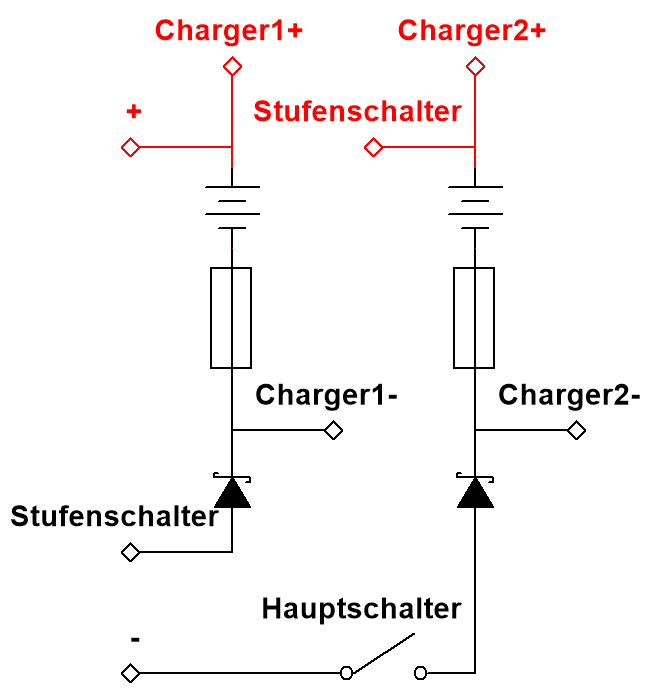
\includegraphics[width=0.45\textwidth]{images/BAT.PNG}
	\caption{Verschaltung Batterie}
	\label{fig:versch_bat}
\end{figure}